\documentclass[11pt]{article}

\usepackage[a4paper,margin=22mm]{geometry}
\usepackage[T1]{fontenc}
\usepackage[utf8]{inputenc}
\usepackage{lmodern}
\usepackage{microtype}
\usepackage{parskip}
\usepackage{enumitem}
\usepackage{booktabs}
\usepackage{tabularx}
\usepackage{array}
\usepackage{xcolor}
\usepackage{graphicx}
\usepackage{float}
\usepackage{fancyhdr}
\usepackage{hyperref}
\usepackage{listings}
\usepackage{tikz}
\usetikzlibrary{arrows.meta,backgrounds,calc,fit,positioning,shapes.geometric}

\definecolor{ink}{HTML}{172033}
\definecolor{muted}{HTML}{5B6475}
\definecolor{blue}{HTML}{2563EB}
\definecolor{bluefill}{HTML}{DBEAFE}
\definecolor{green}{HTML}{15803D}
\definecolor{greenfill}{HTML}{DCFCE7}
\definecolor{amber}{HTML}{B45309}
\definecolor{amberfill}{HTML}{FEF3C7}
\definecolor{purple}{HTML}{7E22CE}
\definecolor{purplefill}{HTML}{F3E8FF}
\definecolor{red}{HTML}{B91C1C}
\definecolor{redfill}{HTML}{FEE2E2}
\definecolor{grayfill}{HTML}{F1F5F9}
\definecolor{linegray}{HTML}{CBD5E1}

\hypersetup{
  colorlinks=true,
  linkcolor=blue,
  urlcolor=blue,
  pdftitle={VideoMASys System Design},
  pdfauthor={VideoMASys Project}
}

\pagestyle{fancy}
\fancyhf{}
\lhead{VideoMASys System Design}
\rhead{Version 0.1}
\cfoot{\thepage}
\setlength{\headheight}{14pt}

\setlist[itemize]{leftmargin=*,itemsep=2pt,topsep=4pt}
\setlist[enumerate]{leftmargin=*,itemsep=2pt,topsep=4pt}

\lstdefinelanguage{json}{
  basicstyle=\ttfamily\small,
  string=[s]{"}{"},
  stringstyle=\color{green!60!black},
  comment=[l]{//},
  commentstyle=\color{muted},
  morecomment=[s]{/*}{*/},
  showstringspaces=false,
  breaklines=true,
  frame=single,
  rulecolor=\color{linegray},
  backgroundcolor=\color{grayfill},
  columns=fullflexible
}

\newcommand{\system}{\textsc{VideoMASys}}
\newcommand{\term}[1]{\textbf{#1}}
\newcommand{\code}[1]{\texttt{#1}}

\tikzset{
  >={Latex[length=2.2mm]},
  box/.style={draw=linegray, rounded corners=2pt, fill=white, align=center,
    minimum height=9mm, minimum width=25mm, inner sep=4pt, font=\small},
  agent/.style={box, draw=blue, fill=bluefill},
  worker/.style={box, draw=purple, fill=purplefill},
  decision/.style={diamond, draw=amber, fill=amberfill, align=center,
    aspect=2.0, inner sep=2pt, font=\small},
  store/.style={cylinder, shape border rotate=90, aspect=0.25,
    draw=green, fill=greenfill, align=center, minimum height=11mm,
    minimum width=24mm, font=\small},
  output/.style={box, draw=green, fill=greenfill},
  guard/.style={box, draw=amber, fill=amberfill},
  danger/.style={box, draw=red, fill=redfill},
  flow/.style={->, thick, draw=ink},
  dataflow/.style={->, draw=muted, dashed},
  group/.style={draw=linegray, rounded corners=4pt, fill=grayfill!45,
    inner sep=7pt}
}

\title{\vspace{-12mm}\textbf{VideoMASys}\\
\large Production-Oriented Multi-Task Video Understanding and Editing System\\[2mm]
\normalsize System Design, Version 0.1}
\author{Architecture proposal based on Structured Video Programming principles}
\date{5 September 2026}

\begin{document}
\maketitle

\begin{abstract}
\system{} is a multi-task video intelligence platform for question answering,
referring-object segmentation, object tracking, and non-destructive video
editing. Its central design is to process a video once, cache a hierarchical
semantic representation, and inspect only the time ranges and pixels required
for each request. A language model supplies task decomposition and semantic
reasoning through a typed plan. Deterministic validators, schedulers, tools, and
renderers execute that plan. This preserves the intelligence of agentic systems
without placing an unbounded chain of model calls or arbitrary generated code on
the production request path.
\end{abstract}

\tableofcontents
\newpage

\section{Executive Summary}

The system is divided into two paths:

\begin{enumerate}
  \item \term{Offline ingestion} converts source media into reusable temporal,
  textual, visual, and object artifacts. It creates video, scene, shot, event,
  transcript, OCR, and keyframe records and indexes their embeddings.
  \item \term{Online task execution} compiles a user request into a bounded,
  typed workflow; retrieves the most relevant cached nodes; and escalates to
  pixel-level analysis only when cached evidence is insufficient.
\end{enumerate}

The architecture deliberately distinguishes an \term{agent} from an LLM call.
An agent is a role with a typed input, typed output, policy, budget, and trace.
Some agents use an LLM, while retrieval, temporal reasoning, media decoding,
mask propagation, tracking, rendering, and most validation remain deterministic
services. In the normal case, a request uses one planning call and at most one
batched visual-model call.

\subsection{Core decisions}

\begin{itemize}
  \item Use an LLM as a semantic planner and bounded replanner.
  \item Generate a typed intermediate representation (IR), not Python or shell.
  \item Use a deterministic compiler, validator, and workflow executor.
  \item Separate reusable video understanding from task-specific execution.
  \item Treat the vector database as a semantic index, not as media storage.
  \item Use PostgreSQL with pgvector for both authoritative metadata and the
  prototype vector index; preserve a \code{VectorIndex} interface for later scale-out.
  \item Keep originals and derived media in object storage; keep durable state in
  a relational database; keep embeddings in a replaceable vector index.
  \item Start as a modular service plus dedicated CPU/GPU workers. Split into
  additional services only when measured scaling requirements justify it.
  \item Make every result reproducible through evidence identifiers, timestamps,
  model versions, plan versions, and an execution trace.
\end{itemize}

\section{Goals and Non-Goals}

\subsection{Goals}

\begin{itemize}
  \item Support multiple tasks through one video representation and tool layer.
  \item Avoid reading or decoding the complete original video at query time.
  \item Provide bounded latency through progressive evidence acquisition.
  \item Support synchronous fast paths and asynchronous long-running jobs.
  \item Allow models, vector stores, and media processors to be replaced behind
  stable interfaces.
  \item Produce inspectable evidence, provenance, confidence, and task artifacts.
  \item Enforce tenant isolation, media access controls, quotas, and safe execution.
\end{itemize}

\subsection{Non-goals for the first release}

\begin{itemize}
  \item Exhaustively detect and track every object in every uploaded video.
  \item Provide frame-perfect professional editing for arbitrary natural-language
  instructions without review.
  \item Permit agents to execute arbitrary source code or invoke unregistered tools.
  \item Guarantee a single model supports every language, domain, and media format.
  \item Begin with a large collection of independently deployed microservices.
\end{itemize}

\section{System Context and Architecture}

Figure~\ref{fig:architecture} shows the common ingestion, planning, evidence,
task, and verification layers. Task branches share the same cached hierarchy and
targeted media-access mechanisms.

\begin{figure}[H]
\centering
\resizebox{0.98\textwidth}{!}{%
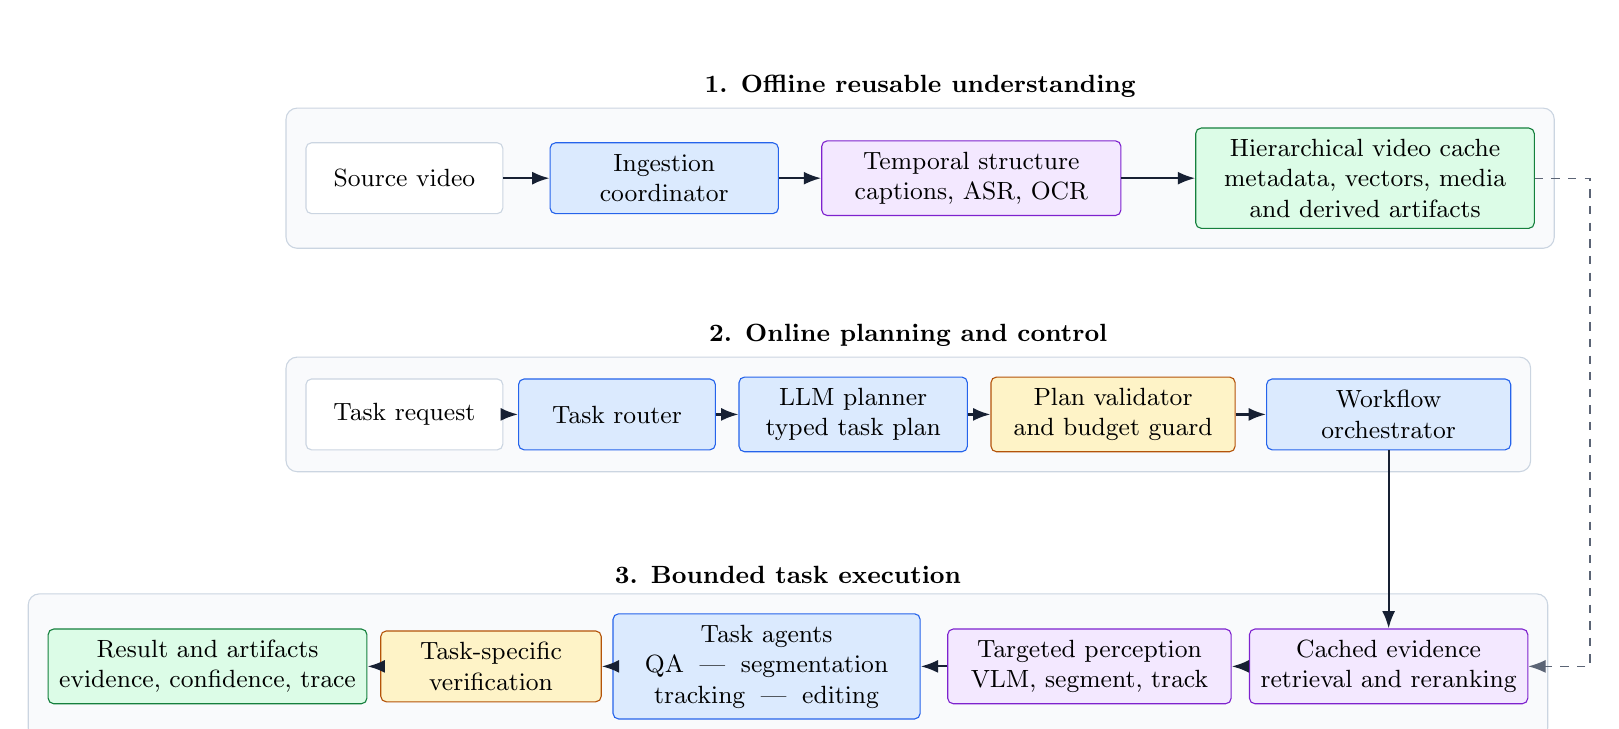
\begin{tikzpicture}[x=1cm,y=1cm]
  % Lane 1: reusable offline understanding (left to right).
  \node[box] (source) at (0,5.2) {Source video};
  \node[agent, minimum width=29mm] (ingest) at (3.3,5.2)
    {Ingestion\\coordinator};
  \node[worker, minimum width=38mm] (structure) at (7.2,5.2)
    {Temporal structure\\captions, ASR, OCR};
  \node[output, minimum width=43mm] (cache) at (12.2,5.2)
    {Hierarchical video cache\\metadata, vectors, media\\and derived artifacts};

  % Lane 2: online control (left to right).
  \node[box] (request) at (0,2.2) {Task request};
  \node[agent] (router) at (2.7,2.2) {Task router};
  \node[agent, minimum width=29mm] (planner) at (5.7,2.2)
    {LLM planner\\typed task plan};
  \node[guard, minimum width=31mm] (validator) at (9.0,2.2)
    {Plan validator\\and budget guard};
  \node[agent, minimum width=31mm] (orch) at (12.5,2.2)
    {Workflow\\orchestrator};

  % Lane 3: bounded execution (right to left).
  \node[worker, minimum width=34mm] (evidence) at (12.5,-1.0)
    {Cached evidence\\retrieval and reranking};
  \node[worker, minimum width=36mm] (perception) at (8.7,-1.0)
    {Targeted perception\\VLM, segment, track};
  \node[agent, minimum width=39mm] (tasks) at (4.6,-1.0)
    {Task agents\\QA \;|\; segmentation\\tracking \;|\; editing};
  \node[guard, minimum width=28mm] (verify) at (1.1,-1.0)
    {Task-specific\\verification};
  \node[output, minimum width=33mm] (result) at (-2.5,-1.0)
    {Result and artifacts\\evidence, confidence, trace};

  \draw[flow] (source) -- (ingest);
  \draw[flow] (ingest) -- (structure);
  \draw[flow] (structure) -- (cache);

  \draw[flow] (request) -- (router);
  \draw[flow] (router) -- (planner);
  \draw[flow] (planner) -- (validator);
  \draw[flow] (validator) -- (orch);

  \draw[flow] (orch) -- (evidence);
  \draw[flow] (evidence) -- (perception);
  \draw[flow] (perception) -- (tasks);
  \draw[flow] (tasks) -- (verify);
  \draw[flow] (verify) -- (result);

  % Cache access is routed around the control lane, never through a block.
  \draw[dataflow] (cache.east) -- ++(7mm,0) |- (evidence.east);

  \begin{scope}[on background layer]
    \node[group, fit=(source)(ingest)(structure)(cache),
      label={[font=\bfseries\small]above:1. Offline reusable understanding}] (offline) {};
    \node[group, fit=(request)(router)(planner)(validator)(orch),
      label={[font=\bfseries\small]above:2. Online planning and control}] (control) {};
    \node[group, fit=(result)(verify)(tasks)(perception)(evidence),
      label={[font=\bfseries\small]above:3. Bounded task execution}] (execution) {};
  \end{scope}
\end{tikzpicture}%
}
\caption{General-purpose architecture. Each swimlane has one flow direction;
the only cross-lane data path is the dashed cache-access route. Blue nodes are
agent roles, purple nodes are workers, and amber nodes enforce policy.}
\label{fig:architecture}
\end{figure}

\subsection{Relationship to Structured Video Programming}

The design retains four useful ideas from StructuredVP: hierarchical cached
video structure, coarse-to-fine evidence selection, typed locate/relate
operations, and explicit program traces. It generalizes those ideas beyond QA
and segmentation and changes the execution model for production use:

\begin{itemize}
  \item A task plan is declarative IR rather than generated Python.
  \item Tool calls are registered, typed, permissioned, metered, and cancellable.
  \item Plans and results are durable jobs rather than state held only in one
  WebSocket connection.
  \item Object nodes may be materialized lazily and reused by later tasks.
  \item Editing produces a validated edit decision list before any rendering.
\end{itemize}

\subsection{Prototype model-serving strategy}

The local prototype uses one instruction-tuned \term{Qwen3-VL} checkpoint as
the shared reasoning and visual-language model. It is hosted by vLLM and exposed
through an OpenAI-compatible \code{/v1/chat/completions} endpoint. A VideoMASys
\code{ModelGateway} is the only component allowed to call that endpoint; agents
depend on the gateway interface rather than on vLLM, Qwen-specific request
objects, or a hard-coded base URL. Qwen3-VL is used instead of the text-only
Qwen3 family because ingestion and evidence roles must accept images or sampled
video.

All model-backed roles share the server but retain separate system prompts,
Pydantic response schemas, token limits, temperatures, deadlines, priorities,
and trace labels. The gateway requests JSON-schema-constrained output for plans,
scene/event descriptions, evidence observations, edit decisions, and verifier
decisions. This keeps role behavior independently testable while allowing vLLM
to batch requests against one resident model.

\begin{table}[H]
\centering
\small
\begin{tabularx}{\textwidth}{>{\bfseries}p{34mm} p{48mm} X}
\toprule
Role & Model input & Structured output \\
\midrule
Scene/event analyst & Candidate shot boundaries plus uniformly sampled proxy
frames & Semantic scene/event ranges, labels, boundary confidence \\
Captioner & Frames or a short proxy clip from one bounded node & Caption,
entities, actions, salient text, confidence \\
Planner/replanner & User intent, task schema, cache summary, budgets & Typed task
plan or one bounded plan revision \\
Visual analyst & Question/purpose plus retrieved frames or clips & Evidence
observations tied to timestamps and input artifact IDs \\
Task agents & Validated evidence bundle and requested output contract & Answer,
object prompt, tracking intent, or edit decision list \\
Verifier & Plan, evidence, output, and task-specific checks & Accept, partial,
reject, or bounded evidence-expansion request \\
\bottomrule
\end{tabularx}
\caption{Prototype roles served by one Qwen3-VL endpoint.}
\end{table}

Media probing, decoding, and initial shot-change detection remain deterministic.
They generate bounded candidate windows for the scene/event analyst, so the VLM
does not ingest an entire long source video in one request. Pixel masks, temporal
mask propagation, identity tracking, embeddings, and rendering remain registered
specialist tools: a general VLM may select and parameterize these tools but does
not replace their pixel-accurate outputs.

This single-model arrangement is a prototype optimization, not a permanent
coupling. The gateway records latency, tokens, visual inputs, failures, and
quality by role. A later deployment can route any role to a different local or
hosted API without changing plans, agent schemas, or orchestration code.

\section{Hierarchical Video Cache}

The cache is a graph with a dominant temporal hierarchy rather than a single
flat embedding collection. Nodes carry stable identifiers and can reference
derived artifacts without embedding large binary payloads in the database.

\begin{figure}[H]
\centering
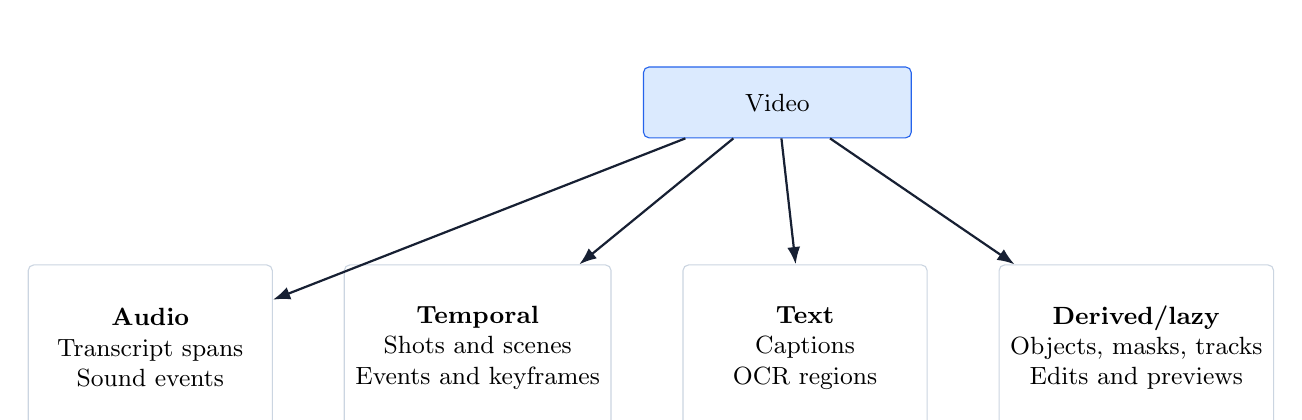
\begin{tikzpicture}[node distance=13mm and 9mm]
  \node[agent, minimum width=34mm] (video) {Video};
  \node[box, below left=16mm and 47mm of video, minimum width=31mm,
    minimum height=21mm] (audio) {\textbf{Audio}\\Transcript spans\\Sound events};
  \node[box, right=of audio, minimum width=31mm, minimum height=21mm]
    (temporal) {\textbf{Temporal}\\Shots and scenes\\Events and keyframes};
  \node[box, right=of temporal, minimum width=31mm, minimum height=21mm]
    (text) {\textbf{Text}\\Captions\\OCR regions};
  \node[box, right=of text, minimum width=31mm, minimum height=21mm]
    (derived) {\textbf{Derived/lazy}\\Objects, masks, tracks\\Edits and previews};

  \draw[flow] (video) -- (audio);
  \draw[flow] (video) -- (temporal);
  \draw[flow] (video) -- (text);
  \draw[flow] (video) -- (derived);
\end{tikzpicture}
\caption{Logical cached representation. Objects, masks, tracks, and editing
artifacts are created lazily unless a deployment explicitly enables eager
processing for a domain.}
\label{fig:hierarchy}
\end{figure}

\subsection{Canonical node model}

Every searchable node should contain:

\begin{itemize}
  \item \code{id}, \code{tenant\_id}, \code{video\_id}, \code{parent\_id}, and
  \code{node\_type};
  \item half-open time range \code{[start\_ms, end\_ms)} and optional frame range;
  \item text description, transcript text, OCR text, and structured attributes;
  \item pointers to keyframes, proxy clips, masks, tracks, or render outputs;
  \item embedding references and lexical-index fields;
  \item model, prompt, preprocessing, and schema versions;
  \item content hash, creation time, quality score, and provenance.
\end{itemize}

Half-open millisecond intervals are canonical. Frame numbers are auxiliary
because variable-frame-rate media and transcoded proxies do not preserve one
universal frame index.

\subsection{Storage responsibilities}

\begin{table}[ht]
\centering
\begin{tabularx}{\textwidth}{>{\bfseries}p{28mm} X X}
\toprule
Store & Owns & Does not own \\
\midrule
Object storage & Originals, proxy clips, keyframes, audio, masks, overlays,
rendered edits & Workflow state or searchable metadata \\
Relational DB & Tenants, videos, temporal nodes, task jobs, plans, leases,
lineage, permissions & Large media blobs \\
Vector index & Embeddings and filterable identifiers for semantic retrieval &
Authoritative metadata or media \\
Artifact cache & Versioned VLM observations, decoded ranges, mask propagation,
tracks, retrieval and answer results & The only durable copy of results \\
\bottomrule
\end{tabularx}
\caption{Storage boundaries. The vector index is a derived, rebuildable index.}
\end{table}

\subsection{Prototype database choice}

The prototype uses PostgreSQL with pgvector. Video hierarchy, temporal ranges,
jobs, plans, permissions, provenance, and embedding rows remain transactionally
consistent in one service. B-tree indexes cover tenant/video/type filters, GiST
indexes cover temporal overlap, GIN indexes cover JSON and lexical fields, and
HNSW indexes cover text and visual embeddings. The application accesses vector
search through a \code{VectorIndex} port rather than issuing pgvector-specific
queries outside the storage adapter.

Milvus is a later scale-out option, not an authoritative store. If benchmarks
show that vector retrieval misses its latency objective at the required vector
count or query concurrency, an outbox-driven indexer can project immutable node
IDs and embeddings from PostgreSQL into Milvus. Search results are then hydrated
and authorized from PostgreSQL. This preserves one source of truth and makes the
external vector index rebuildable.

\section{Agents, Tools, and Responsibilities}

\subsection{Agent contract}

Each agent has a narrow contract:

\begin{itemize}
  \item versioned input and output schemas;
  \item allowed tools and data scopes;
  \item latency, token, frame, duration, and monetary budgets;
  \item retry and fallback policy;
  \item deterministic correlation identifiers and trace events;
  \item explicit confidence and failure categories.
\end{itemize}

Agents do not communicate through unbounded conversational transcripts. They
exchange state through a task context and immutable, typed evidence records.

\subsection{Core roles}

\begin{table}[ht]
\centering
\small
\begin{tabularx}{\textwidth}{>{\bfseries}p{31mm} p{28mm} X}
\toprule
Role & Implementation & Responsibility \\
\midrule
Ingestion coordinator & Deterministic workflow & Schedules probing,
transcoding, temporal structuring, descriptions, embeddings, and indexing. \\
Task router & Rules or small model & Classifies task type, synchrony, and likely
cost; direct-routes simple operations. \\
Planner & LLM with structured output & Decomposes complex intent into typed,
bounded operations and declares required output. \\
Plan validator/compiler & Deterministic & Type-checks the graph, validates
permissions and budgets, resolves tool versions, and creates executable jobs. \\
Retrieval agent & Deterministic search/rerank & Searches captions, transcripts,
OCR, temporal nodes, and cached object artifacts. \\
Visual analyst & VLM worker & Examines only selected keyframes or proxy clips and
emits observations with temporal provenance. \\
Object specialist & Vision workers & Detects, segments, propagates, tracks, and
re-identifies objects within bounded ranges. \\
QA agent & LLM or deterministic function & Answers from an evidence bundle;
handles counting and comparison deterministically where possible. \\
Editing agent & LLM plus deterministic compiler & Produces a typed edit decision
list; never emits executable shell commands. \\
Verifier & Rules, metrics, optional model & Checks evidence sufficiency and
task-specific output validity; may request one bounded expansion. \\
\bottomrule
\end{tabularx}
\caption{Agent roles. An agent is an operational boundary, not necessarily a
separate language-model invocation.}
\end{table}

\section{Typed Task Plan}

The planner returns a directed acyclic graph expressed as versioned JSON. The
plan separates \term{evidence operations}, which discover or materialize facts,
from \term{task operations}, which produce an answer or artifact.

\subsection{Example plan}

\begin{lstlisting}[language=json,caption={Illustrative plan for a tracking request.}]
{
  "schema_version": "1.0",
  "task": "object_tracking",
  "video_ids": ["vid_01"],
  "steps": [
    {
      "id": "find_seed",
      "operator": "search_events",
      "inputs": [],
      "arguments": {"query": "red car enters the junction", "limit": 3}
    },
    {
      "id": "inspect_seed",
      "operator": "inspect_visual",
      "inputs": ["find_seed"],
      "arguments": {"purpose": "localize the red car"}
    },
    {
      "id": "track",
      "operator": "track_object",
      "inputs": ["inspect_seed"],
      "arguments": {"direction": "both", "max_duration_ms": 90000}
    },
    {
      "id": "verify",
      "operator": "verify_track",
      "inputs": ["track"],
      "arguments": {"minimum_continuity": 0.85}
    }
  ],
  "output": {"from": "verify", "format": "track_json_and_overlay"},
  "budget": {"deadline_ms": 30000, "max_visual_seconds": 90,
             "max_replans": 1}
}
\end{lstlisting}

\subsection{Initial operator set}

\begin{itemize}
  \item Retrieval: \code{search\_videos}, \code{search\_scenes},
  \code{search\_events}, \code{search\_transcript}, \code{search\_ocr}.
  \item Temporal: \code{before}, \code{after}, \code{around},
  \code{overlap}, \code{within}, \code{expand\_range}, \code{merge\_ranges}.
  \item Media: \code{fetch\_keyframes}, \code{decode\_range},
  \code{sample\_frames}, \code{inspect\_visual}.
  \item Objects: \code{detect\_object}, \code{segment\_object},
  \code{propagate\_mask}, \code{track\_object}, and
  \code{reidentify\_\allowbreak object}.
  \item QA: \code{count}, \code{compare}, \code{aggregate\_evidence},
  \code{compose\_answer}, \code{verify\_answer}.
  \item Editing: \code{select\_ranges}, \code{trim}, \code{concat},
  \code{crop}, \code{overlay}, \code{replace\_audio},
  \code{compile\_timeline}, \code{render}, \code{verify\_render}.
\end{itemize}

Every operator declares accepted input types, output type, side effects, cost
class, cache behavior, and whether it may run synchronously. Unknown operators,
cycles, invalid references, and over-budget plans are rejected before execution.

\section{Common Evidence Pipeline}

The orchestrator first attempts to satisfy a task from cached textual and visual
evidence. It progressively acquires more expensive evidence only when the plan
or verifier requires it.

\begin{figure}[H]
\centering
\resizebox{0.90\textwidth}{!}{%
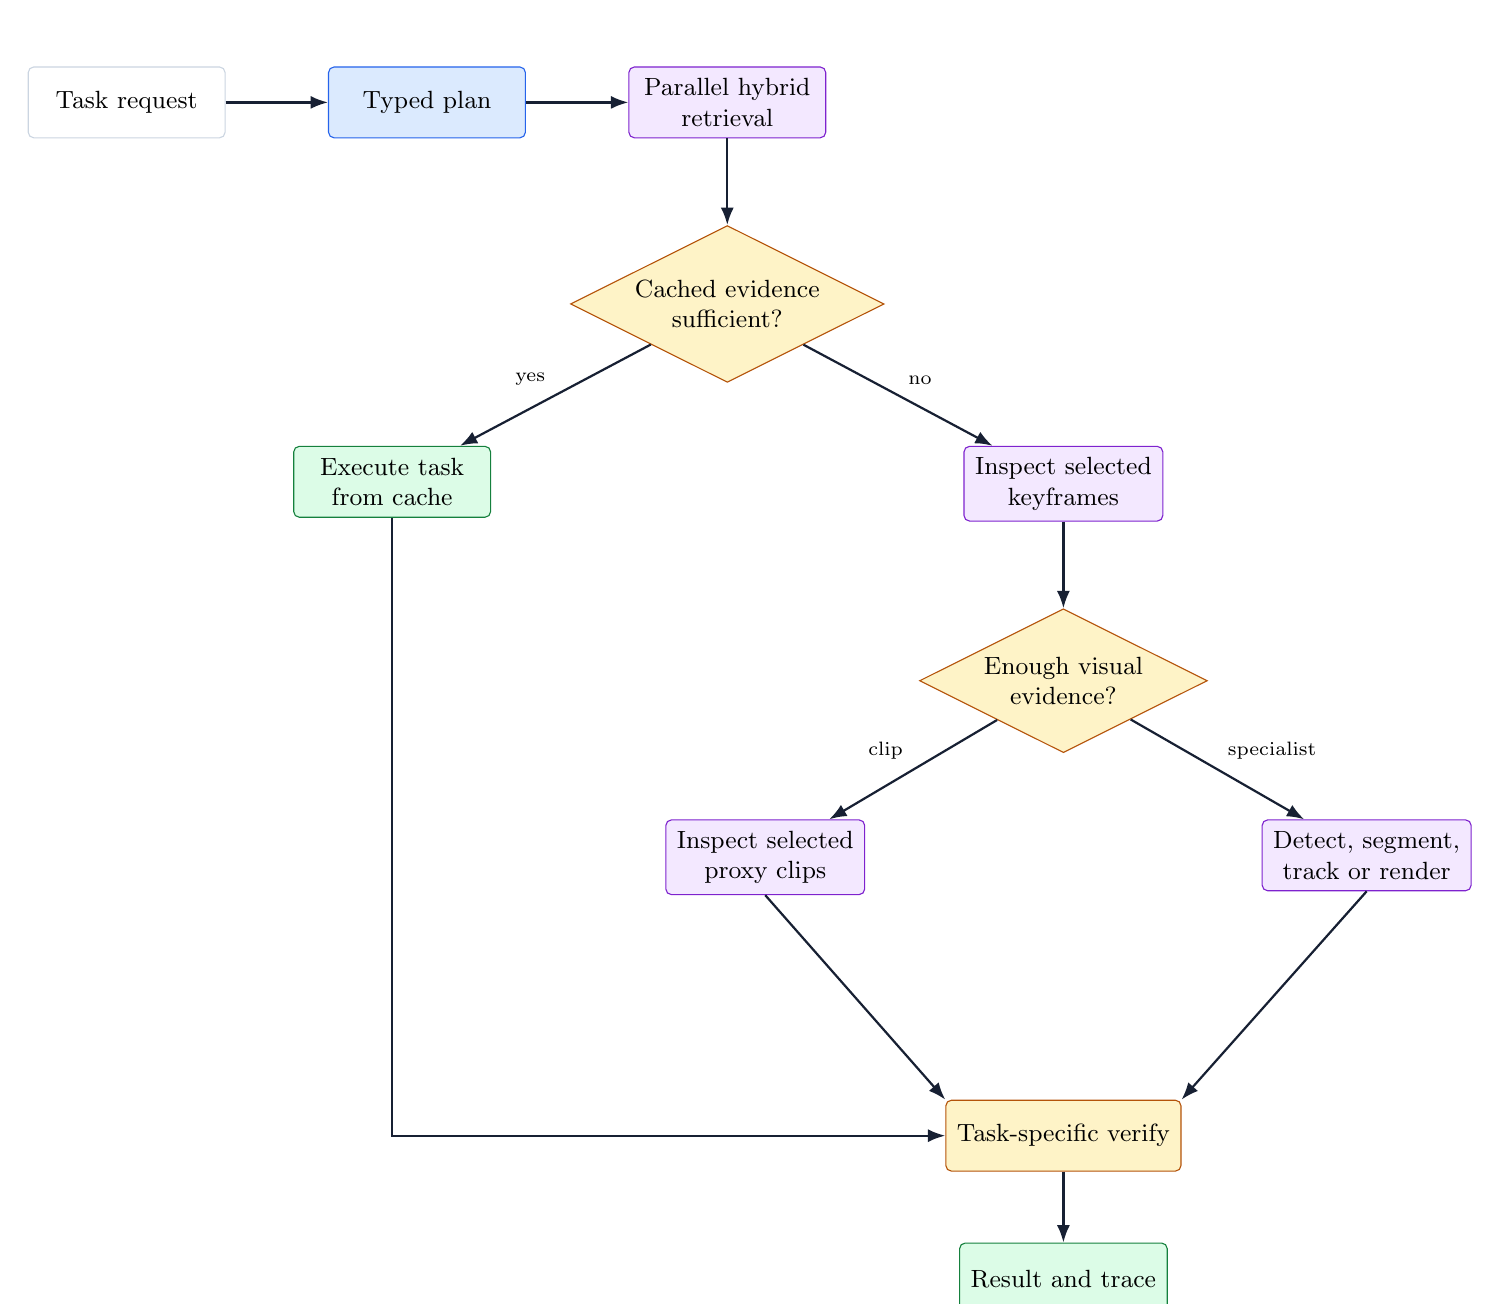
\begin{tikzpicture}[node distance=9mm and 13mm]
  \node[box] (query) {Task request};
  \node[agent, right=of query] (plan) {Typed plan};
  \node[worker, right=of plan] (search) {Parallel hybrid\\retrieval};
  \node[decision, below=11mm of search] (cached) {Cached evidence\\sufficient?};

  \node[output, below left=13mm and 20mm of cached] (fast) {Execute task\\from cache};
  \node[worker, below right=13mm and 20mm of cached] (frames) {Inspect selected\\keyframes};
  \node[decision, below=11mm of frames] (enough) {Enough visual\\evidence?};
  \node[worker, below left=13mm and 16mm of enough] (clip) {Inspect selected\\proxy clips};
  \node[worker, below right=13mm and 16mm of enough] (deep) {Detect, segment,\\track or render};
  \node[guard, below=44mm of enough] (verify) {Task-specific verify};
  \node[output, below=of verify] (result) {Result and trace};

  \draw[flow] (query) -- (plan);
  \draw[flow] (plan) -- (search);
  \draw[flow] (search) -- (cached);
  \draw[flow] (cached) -- node[above left, font=\scriptsize]{yes} (fast);
  \draw[flow] (cached) -- node[above right, font=\scriptsize]{no} (frames);
  \draw[flow] (frames) -- (enough);
  \draw[flow] (enough) -- node[above left, font=\scriptsize]{clip} (clip);
  \draw[flow] (enough) -- node[above right, font=\scriptsize]{specialist} (deep);
  \draw[flow] (fast.south) |- (verify.west);
  \draw[flow] (clip.south) -- (verify.north west);
  \draw[flow] (deep.south) -- (verify.north east);
  \draw[flow] (verify) -- (result);
\end{tikzpicture}%
}
\caption{Progressive evidence acquisition. The common path stays cheap; deep
perception and rendering are explicit escalation paths. The verifier may request
one bounded evidence expansion through the orchestrator.}
\label{fig:escalation}
\end{figure}

\subsection{Retrieval strategy}

\begin{enumerate}
  \item Apply tenant, video, time, language, and node-type filters.
  \item Search dense embeddings and lexical fields in parallel.
  \item Fuse and deduplicate results, preserving parent/child relationships.
  \item Rerank a small candidate set using query--caption relevance and temporal
  constraints.
  \item Add bounded neighboring context around strong matches.
  \item Return an evidence bundle with scores, timestamps, descriptions, and
  artifact pointers---not full video bytes.
\end{enumerate}

Initial defaults should cap retrieval at 20 candidates, visual inspection at
three ranges, combined decoded duration at 60 seconds, sampled frames at 32,
and replanning at one attempt. These are deployment defaults rather than values
embedded in the plan schema.

\section{Task Workflows}

\subsection{Video question answering}

The planner identifies whether the question is factual, temporal, causal,
counting, comparative, or object-centric. Transcript, OCR, captions, and event
nodes are retrieved first. A visual analyst receives a single batch containing
the selected evidence. Counting, sorting, and simple comparisons are performed
by deterministic operators when their inputs are reliable. The result contains
an answer, confidence, supporting node IDs, timestamps, and limitations.

\subsection{Referring-object segmentation}

The system retrieves likely temporal windows before invoking segmentation. A
visual grounding step chooses one or more seed frames and object prompts. A
segmentation worker generates seed masks, and a propagation worker extends them
through the requested interval. The verifier checks mask continuity, area jumps,
boundary confidence, and prompt consistency. Outputs may include run-length
encoded masks, alpha video, overlays, and quality metrics.

\subsection{Object tracking}

Tracking begins from a grounded seed rather than scanning the full video by
default. Propagation proceeds within a bounded interval, with re-identification
at scene cuts or after loss. Long videos are divided into jobs that can run in
parallel and merge through identity constraints. Outputs include timestamped
boxes or masks, confidence, visibility state, and an optional overlay video.

\subsection{Video editing}

Editing is non-destructive. The editing agent converts natural-language intent
into a typed edit decision list (EDL) referencing source assets and half-open
time ranges. The compiler validates bounds, codecs, transitions, output aspect
ratio, and overlay assets. A deterministic renderer produces a preview and then
the final artifact. The system retains the EDL, render manifest, source hashes,
and media-tool version so an edit can be reproduced.

Examples include semantic highlight extraction, removal of matching scenes,
object-focused crops, reframing around a track, subtitle insertion, and audio
replacement. Destructive overwrite of source media is prohibited.

\section{Caching and Reuse}

\subsection{Cache levels}

\begin{enumerate}
  \item \term{Ingestion cache}: probes, scene boundaries, transcripts, OCR,
  captions, keyframes, and embeddings.
  \item \term{Evidence cache}: query retrieval results and bounded VLM
  observations for a video range.
  \item \term{Object cache}: detections, seed masks, propagated masks, tracklets,
  and re-identification embeddings.
  \item \term{Task cache}: validated answers, segmentation exports, track exports,
  EDLs, previews, and final renders.
\end{enumerate}

A cache key must include the tenant scope, content hash, exact time range, input
parameters, model identifier, model revision, prompt revision, preprocessing
revision, and output schema version. Cache writes should use single-flight
deduplication so concurrent identical requests do not repeat GPU work.

\subsection{Invalidation}

Artifacts are immutable. A new model or preprocessing version writes a new
artifact rather than mutating the old one. Database pointers identify the
active version. Garbage collection deletes unreferenced derived artifacts only
after a retention period; source-media deletion follows tenant policy and is
separately audited.

\section{Latency and Efficiency}

\subsection{Service classes}

\begin{table}[ht]
\centering
\begin{tabularx}{\textwidth}{>{\bfseries}p{32mm} p{28mm} X}
\toprule
Class & Initial objective & Typical use \\
\midrule
Interactive cache & p95 below 2 s & Metadata, transcript, OCR, or sufficiently
descriptive cached nodes \\
Interactive visual & p95 below 8 s & QA or localization using one batched set of
keyframes/proxy clips \\
Deep perception & Job accepted below 1 s; completion target 10--60 s &
Segmentation and bounded tracking \\
Render & Job accepted below 1 s; duration-dependent completion & Editing,
overlay generation, transcoding, and long-video tracking \\
\bottomrule
\end{tabularx}
\caption{Latency objectives are starting SLOs and must be calibrated against
chosen models, media duration, output resolution, and hardware.}
\end{table}

\subsection{Primary optimizations}

\begin{itemize}
  \item Keep models resident in dedicated workers; never load them per request.
  \item Batch all selected frames or clips for a task into one visual call.
  \item Decode low-resolution proxy media first and originals only when output
  quality requires them.
  \item Run independent lexical, vector, metadata, transcript, and OCR searches
  concurrently.
  \item Use dynamic batching and length-aware queues for GPU inference.
  \item Route simple plans to rules or small models and complex plans to a
  stronger planner.
  \item Apply backpressure at admission and queue boundaries rather than allowing
  unbounded GPU queues.
  \item Propagate deadlines and cancellation tokens through every operation.
  \item Use semantic result caches carefully; never cross tenant or permission
  scopes.
\end{itemize}

\section{APIs and Job Lifecycle}

\subsection{External API}

An initial HTTP API should expose:

\begin{itemize}
  \item \code{POST /v1/videos}: register an object URI or begin an upload;
  \item \code{GET /v1/videos/\{id\}}: metadata and ingestion readiness;
  \item \code{POST /v1/tasks}: submit any supported task with constraints;
  \item \code{GET /v1/tasks/\{id\}}: status, progress, result, and errors;
  \item \code{GET /v1/tasks/\{id\}/events}: server-sent progress events;
  \item \code{POST /v1/tasks/\{id\}/cancel}: cooperative cancellation;
  \item \code{GET /v1/artifacts/\{id\}}: authorized artifact metadata and a
  short-lived download URL.
\end{itemize}

\subsection{Unified task request}

\begin{lstlisting}[language=json]
{
  "task_type": "qa | segmentation | tracking | editing",
  "video_ids": ["vid_01"],
  "instruction": "Track the cyclist and blur their face",
  "constraints": {
    "time_range_ms": [0, 120000],
    "latency_class": "balanced",
    "maximum_visual_seconds": 60
  },
  "output": {
    "formats": ["track_json", "edited_mp4"],
    "include_trace": true
  },
  "idempotency_key": "client-generated-key"
}
\end{lstlisting}

\subsection{Lifecycle}

Jobs transition through \code{accepted}, \code{planning}, \code{retrieving},
\code{executing}, \code{verifying}, and a terminal state of \code{succeeded},
\code{partially\_succeeded}, \code{failed}, or \code{cancelled}. Step attempts,
leases, and outputs are durable. Workers must be idempotent because a lease can
expire and a step can be retried.

\section{Deployment and Scaling}

\subsection{Initial topology}

The first production-like deployment should be intentionally small:

\begin{itemize}
  \item one stateless API/orchestrator service;
  \item PostgreSQL for metadata, jobs, plans, and leases;
  \item a vector index behind a repository interface;
  \item S3-compatible object storage;
  \item a durable task queue;
  \item CPU media workers for probing, slicing, and rendering;
  \item one or more persistent GPU model workers;
  \item OpenTelemetry-compatible traces, metrics, and structured logs.
\end{itemize}

This can be deployed locally with containers and in production with the same
logical components. Separate planner, retrieval, object, and rendering services
only when they require independent scaling, fault isolation, or ownership.

\subsection{Scheduling}

Queues should be split by resource class: short CPU, long CPU/render, small GPU,
large GPU, and latency-sensitive GPU. Admission control estimates cost from
video duration, selected ranges, resolution, model, and output format. Tenant
quotas constrain concurrent tasks, stored bytes, GPU seconds, and planner tokens.

\section{Reliability, Security, and Safety}

\begin{itemize}
  \item Authenticate every API call and authorize every video and artifact.
  \item Use scoped object-store URLs with short expiry; do not give model workers
  general storage credentials.
  \item Validate MIME type and media structure, enforce byte/duration limits, and
  isolate media parsers and renderers.
  \item Execute only registered operators. Generated Python, imports, shell
  commands, arbitrary URLs, and arbitrary filesystem paths are not plan features.
  \item Keep source media immutable and require a new artifact ID for every edit.
  \item Apply per-step timeouts, memory limits, cancellation, retries with jitter,
  and circuit breakers around external model providers.
  \item Redact secrets and signed URLs from logs and model prompts.
  \item Record who requested an edit, which inputs were used, and which artifact
  was produced.
  \item Make partial success explicit, especially for occluded tracks or
  low-confidence masks.
\end{itemize}

\section{Observability and Evaluation}

Each task creates a trace rooted at \code{task\_id}. Spans include planning,
validation, each retrieval source, reranking, media fetch/decode, model queue and
inference time, cache access, task execution, verification, and artifact upload.

Core operational metrics include:

\begin{itemize}
  \item end-to-end p50/p95/p99 latency by task and service class;
  \item queue wait, model inference, decoded seconds, sampled frames, and GPU
  seconds per task;
  \item cache hit rate at each cache level;
  \item plan validation failure and replan rate;
  \item evidence expansion rate and retrieved-duration ratio;
  \item task success, partial success, cancellation, and failure categories;
  \item cost per successful task and artifact storage growth.
\end{itemize}

Quality evaluation is task-specific:

\begin{itemize}
  \item QA: exact/fuzzy accuracy, evidence recall, timestamp precision, and
  calibration;
  \item segmentation: region and boundary metrics, temporal consistency, and
  identity-switch rate;
  \item tracking: HOTA/ID-style metrics, track continuity, and recovery after
  occlusion or scene cuts;
  \item editing: instruction satisfaction, edit-boundary accuracy, render
  validity, preservation of unedited content, and human preference.
\end{itemize}

Every benchmark should also report latency, GPU seconds, planner tokens, decoded
video duration, and cache state. Accuracy without cost and latency is not an
adequate measure of this system.

\section{Implementation Roadmap}

\subsection{Phase 1: Foundation and vertical slice}

\begin{itemize}
  \item Establish package boundaries, configuration, schemas, and local services.
  \item Register video, ingest scenes/keyframes/transcript/captions, and index
  nodes.
  \item Implement typed plans, validator, tool registry, job state, and traces.
  \item Deliver QA from cached evidence plus targeted keyframes.
\end{itemize}

\subsection{Phase 2: Object intelligence}

\begin{itemize}
  \item Add object grounding, seed masks, mask propagation, and track storage.
  \item Deliver referring segmentation and bounded tracking.
  \item Add object-artifact reuse and task-specific verification.
\end{itemize}

\subsection{Phase 3: Editing}

\begin{itemize}
  \item Define the edit decision list and deterministic compiler.
  \item Add preview rendering, artifact lineage, and render validation.
  \item Support semantic cuts, concatenation, reframing from tracks, blur,
  subtitles, overlays, and audio operations.
\end{itemize}

\subsection{Phase 4: Production hardening}

\begin{itemize}
  \item Add authentication, tenant quotas, retention policy, load tests, disaster
  recovery, autoscaling, and deployment automation.
  \item Calibrate routing and confidence thresholds from benchmark and production
  traces.
  \item Introduce additional service separation only where measurements justify it.
\end{itemize}

\section{Initial Acceptance Criteria}

The first integrated release is acceptable when it can:

\begin{enumerate}
  \item ingest a video asynchronously and expose a versioned hierarchy;
  \item answer a question using no more than three retrieved ranges and return
  timestamped evidence;
  \item segment and track a referred object over a bounded interval and cache the
  resulting masks or tracks;
  \item compile an editing instruction to an inspectable EDL and render a new,
  non-destructive artifact;
  \item reject invalid or over-budget plans before execution;
  \item resume or safely retry work after a worker failure;
  \item show a trace that connects the request, plan, evidence, model/tool
  versions, task output, and final artifact;
  \item enforce that one tenant cannot retrieve another tenant's media, vectors,
  metadata, or cached artifacts.
\end{enumerate}

\section{Open Decisions}

The implementation phase should resolve these choices through small benchmarks:

\begin{itemize}
  \item the measured vector-count, concurrency, recall, and latency threshold at
  which the \code{VectorIndex} implementation should move from pgvector to Milvus;
  \item the Qwen3-VL checkpoint size, quantization, context limit, and vLLM
  concurrency settings for the available prototype hardware;
  \item the first replacement targets and routing policy behind the model gateway;
  \item mask propagation, tracking, and re-identification model families;
  \item proxy resolutions and frame-sampling policy by content domain;
  \item synchronous limits and default budgets per task;
  \item media renderer and the exact versioned EDL schema.
\end{itemize}

These are replaceable implementation decisions. The stable architectural
contract is the typed plan, shared evidence model, hierarchical cache, bounded
tool execution, immutable artifacts, and full provenance.

\end{document}
